\subsection{Algoritmo genético}
Para esta práctica se desarrolló un algoritmo genético que se apega al proceso mostrado en la Figura \ref{fig:AG}.

\begin{figure}[htbp]
	\centering
	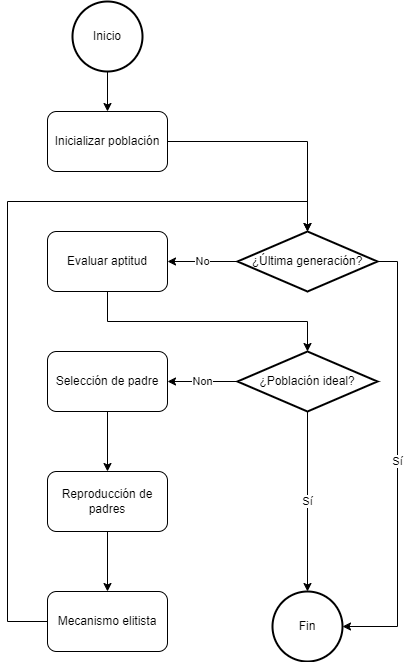
\includegraphics[width=0.5\textwidth]{algoritmo_genetico_proceso}
	\caption{Diagrama de flujo del algoritmo genético implementado.}
	\label{fig:AG}
\end{figure}

Para llevar a cabo dicho proceso, se optó por utilizar el lenguaje de programación Python, donde se diseñaron métodos genéricos para realizar los procesos de generación de población, evaluación de aptitud, selección de individuos, reproducción de individuos, mutación y mecanismos elitistas.

\subsection{Implementación en Python}

\subsubsection{Inicializador de población}
\begin{minted}
[
baselinestretch=1.2,
fontsize=\footnotesize,
linenos
]
{python}
def int_to_oct_array(number: int, padding: int = 8):
    oct_str = oct(number)[2:].zfill(padding)
    oct_array = np.zeros(padding)
    for idx in range(padding):
        oct_array[idx] = oct_str[idx]

    return oct_array


def oct_array_to_int(oct_array: np.ndarray):
    n = oct_array.shape[0]
    pows = [8**pow for pow in range(n)]
    pows = np.array(pows[::-1])
    int_number = np.dot(oct_array, pows)

    return int_number


def init_octal_population(n: int = 10, genes: int = 10):
    min_octal = 0o0
    max_octal = 0o7 * (8**genes) 
    population = np.random.randint(min_octal, max_octal, n, dtype=np.uint64)
    population = [int_to_oct_array(individue, genes) for individue in population]
    population = np.array(population)

    return population
\end{minted}

\newpage
\subsubsection{Evaluación de individuos}
\begin{minted}
[
baselinestretch=1.2,
fontsize=\footnotesize,
linenos
]
{python}
def aptitude_function(x1, x2):
    return 100*(x2 - x1**2)**2 + (x1 - 1)**2


def decode_individue(individue: np.ndarray):
    min_domain = -5
    max_domain = 10
    bits = individue.shape[0]
    min_octal = 0
    max_octal = 8**bits - 1
    decoded_individue = oct_array_to_int(individue)
    decoded_individue = (decoded_individue - min_octal) / (max_octal - min_octal)
    decoded_individue = (max_domain - min_domain) * decoded_individue + min_domain

    return decoded_individue


def evaluate_individue(x1: np.ndarray, x2: np.ndarray):
    x1_decoded = decode_individue(x1)
    x2_decoded = decode_individue(x2)
    aptitude = aptitude_function(x1_decoded, x2_decoded)
    
    return aptitude


def evaluate_population(p_x1: np.ndarray, p_x2: np.ndarray, desc: bool = False):
    aptitudes = np.vstack([evaluate_individue(x1, x2) for x1, x2 in zip(p_x1, p_x2)])
    
    direction = -1 if desc else 1
    sorted_indexes = aptitudes[:, -1].argsort()[::direction]
    sorted_px1 = p_x1[sorted_indexes]
    sorted_px2 = p_x2[sorted_indexes]
    sorted_aptitudes = aptitudes[sorted_indexes]
    avg_aptitude = np.mean(sorted_aptitudes)
    best_aptitude = np.min(sorted_aptitudes)

    return sorted_px1, sorted_px2, sorted_aptitudes, avg_aptitude, best_aptitude
\end{minted}

\subsubsection{Selección de parejas}
\begin{minted}
[
baselinestretch=1.2,
fontsize=\footnotesize,
linenos
]
{python}
def roulette_selection(aptitudes: np.ndarray):
    max_aptitude = np.max(aptitudes)
    fitness = max_aptitude - aptitudes
    total_fitness = fitness.sum()

    couples = []
    couple = []

    for _ in range(aptitudes.shape[0]):
        accumulated = 0
        selection = np.random.uniform(0, total_fitness)

        for idx, aptitude  in enumerate(fitness):
            accumulated += aptitude
            if accumulated >= selection:
                couple.append(idx)
                break
        
        if len(couple) == 2:
            couples.append(couple)
            couple = []

    return np.vstack(couples)
\end{minted}

\subsubsection{Reproducción de individuos}
\begin{minted}
[
baselinestretch=1.2,
fontsize=\footnotesize,
linenos
]
{python}
def two_point_crossover(population: np.ndarray, parents: np.ndarray):
    childrens = np.empty_like(population)
    for idx, couple in enumerate(parents):
        crossover_point = population.shape[1]//3
        childrens[idx*2, :crossover_point] = population[couple[0], :crossover_point]
        childrens[idx*2, crossover_point:2*crossover_point] = population[couple[1], crossover_point:2*crossover_point]
        childrens[idx*2, 2*crossover_point:] = population[couple[0], 2*crossover_point:]
        childrens[idx*2+1, :crossover_point] = population[couple[1], :crossover_point]
        childrens[idx*2+1, crossover_point:2*crossover_point] = population[couple[0], crossover_point:2*crossover_point]
        childrens[idx*2+1, 2*crossover_point:] = population[couple[1], 2*crossover_point:]

    return childrens
\end{minted}

\subsubsection{Mutación}
\begin{minted}
[
baselinestretch=1.2,
fontsize=\footnotesize,
linenos
]
{python}
def scramble_mutation(individues_x1: np.ndarray, individues_x2: np.ndarray, mr: float = 0.10):
    total_individues = individues_x1.shape[0]
    individue_len = individues_x1.shape[1]
    to_mutate = np.random.choice(total_individues, int(total_individues * mr))

    for idx in to_mutate:
        idx_l, idx_r = sorted(np.random.choice(individue_len, 2))
        idx_r = idx_r if idx_r == individue_len else idx_r + 1
        individues_x1[idx][idx_l:idx_r] = np.random.shuffle(individues_x1[idx][idx_l:idx_r][::-1])
        individues_x2[idx][idx_l:idx_r] = np.random.shuffle(individues_x2[idx][idx_l:idx_r][::-1])

    return individues_x1, individues_x2
\end{minted}

\subsubsection{Elitismo}
\begin{minted}
[
baselinestretch=1.2,
fontsize=\footnotesize,
linenos
]
{python}
def genetic_competence(p_x1: np.ndarray, p_x2: np.ndarray, c_x1: np.ndarray, c_x2: np.ndarray):
    all_px1 = np.vstack([p_x1, c_x1])
    all_px2 = np.vstack([p_x2, c_x2])
    sorted_px1, sorted_px2, _, _, _ = evaluate_population(all_px1, all_px2)
    
    return sorted_px1[:p_x1.shape[0]], sorted_px2[:p_x2.shape[0]]
\end{minted}

\subsubsection{Algoritmo completo}
\begin{minted}
[
baselinestretch=1.2,
fontsize=\footnotesize,
linenos
]
{python}
generations = 20

population_x1 = init_octal_population(100, 10)
population_x2 = init_octal_population(100, 10)

last_avg_aptitude = float("inf")
max_stagnant_generations = 2
stagnant_generations = 0
delta = 0.05

avg_aptitudes = []
best_aptitudes = []
evolution = []


for _ in tqdm(range(generations), desc="Generation"):
    population_x1, population_x2, aptitudes, avg_aptitude, best_aptitude = evaluate_population(population_x1, population_x2)
    avg_aptitudes.append(avg_aptitude)
    best_aptitudes.append(best_aptitude)
    evolution.append([population_x1, population_x2, best_aptitude, avg_aptitude])

    if abs(avg_aptitude - last_avg_aptitude) < delta:
        stagnant_generations += 1
        if stagnant_generations > max_stagnant_generations:
            break
    else:
        stagnant_generations = 0

    last_avg_aptitude = avg_aptitude
    parents = roulette_selection(aptitudes)
    childrens_x1 = two_point_crossover(population_x1, parents)
    childrens_x2 = two_point_crossover(population_x2, parents)
    childrens_x1, childrens_x2 = scramble_mutation(childrens_x1, childrens_x2)
    population_x1, population_x2 = genetic_competence(population_x1, population_x2, childrens_x1, childrens_x2)

print(f"Best individue: {decode_individue(evolution[-1][0][0])}, {decode_individue(evolution[-1][1][0])}")
print(f"Best aptitude: {evolution[-1][2]}")
print(f"Avg aptitude: {evolution[-1][3]}")

title = "Roulette selection + two point crossover"
plot_aptitude(avg_aptitudes, best_aptitudes, generations, title)
filename = plot_evolution(evolution, title)
HTML(f'<img src="{filename}">')
\end{minted}

\newpage
\subsection{Pruebas realizadas}
Se implementó una solución en la cuál se utilizan poblaciones con codificación octal, selección mediante el método ruleta, cruza de dos puntos, mutación scramble y competencia genética.

Debido a que el objetivo es determinar un conjunto de soluciones, se realizaron 3 ejecuciones del algoritmo, esto con el objetivo de obtener soluciones posibles al problema.

En cada ejecución del algoritmo se generaron gráficas que muestran el proceso de de evolución, en términos de aptitud y convergencia dentro del espacio de búsqueda.

El criterio de paro utilizado se estableción según los siguientes criterios:

\begin{itemize}
	\item Número de generaciones. Se estableció un límite de 20 generaciones para todos los algoritmos.
	\item Término por $\delta$. Se estableció un valor $\delta=0.05$ con un máximo de 2 generaciones.
\end{itemize}
